\section{Ranking}
Esta funcionalidad es accecida mediante la primera pantalla del programa, dandole click al botón ranking.
\begin{figure}[htbp]
\begin{center}
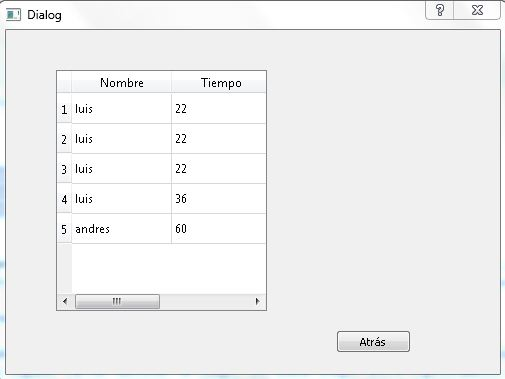
\includegraphics[width=.60\textwidth]{./imagenes/5.jpg}
\caption{Pantalla Ranking}
\label{Pantalla Ranking}
\end{center}
\end{figure}
Esta funcionalidad se la llevo a cabo usando un widget en Qt especial, que nos permitió armar una tabla con los nombres de los jugadores. El ranking es guardado en un archivo de texto ranking.txt, y es cargado en tiempo real a la tabla. Al finalizar el juego de forma satisfactoria el nombre del jugador y el puntaje (número de segundos) son guardados en este archivo.

